%%
%% This is file `sample-acmlarge.tex',
%% generated with the docstrip utility.
%%
%% The original source files were:
%%
%% samples.dtx  (with options: `acmlarge')
%% 
%% IMPORTANT NOTICE:
%% 
%% For the copyright see the source file.
%% 
%% Any modified versions of this file must be renamed
%% with new filenames distinct from sample-acmlarge.tex.
%% 
%% For distribution of the original source see the terms
%% for copying and modification in the file samples.dtx.
%% 
%% This generated file may be distributed as long as the
%% original source files, as listed above, are part of the
%% same distribution. (The sources need not necessarily be
%% in the same archive or directory.)
%%
%% The first command in your LaTeX source must be the \documentclass command.
\documentclass[acmlarge]{acmart}

\def\red#1{\textcolor[rgb]{1,0,0}{#1}}
\usepackage{float}
\usepackage{CJKutf8}
\usepackage{subcaption}
\usepackage{multirow}
\usepackage{url}
\usepackage{appendix}
\usepackage{array, multirow, multicol, rotating, makecell, caption, booktabs}
\usepackage{xcolor,colortbl}

%%
%% \BibTeX command to typeset BibTeX logo in the docs
\AtBeginDocument{%
  \providecommand\BibTeX{{%
    \normalfont B\kern-0.5em{\scshape i\kern-0.25em b}\kern-0.8em\TeX}}}

%% Rights management information.  This information is sent to you
%% when you complete the rights form.  These commands have SAMPLE
%% values in them; it is your responsibility as an author to replace
%% the commands and values with those provided to you when you
%% complete the rights form.
\setcopyright{acmcopyright}
\copyrightyear{2018}
\acmYear{2018}
\acmDOI{10.1145/1122445.1122456}


%%
%% These commands are for a JOURNAL article.
\acmJournal{POMACS}
\acmVolume{37}
\acmNumber{4}
\acmArticle{111}
\acmMonth{8}

%%
%% Submission ID.
%% Use this when submitting an article to a sponsored event. You'll
%% receive a unique submission ID from the organizers
%% of the event, and this ID should be used as the parameter to this command.
%%\acmSubmissionID{123-A56-BU3}

%%
%% The majority of ACM publications use numbered citations and
%% references.  The command \citestyle{authoryear} switches to the
%% "author year" style.
%%
%% If you are preparing content for an event
%% sponsored by ACM SIGGRAPH, you must use the "author year" style of
%% citations and references.
%% Uncommenting
%% the next command will enable that style.
%%\citestyle{acmauthoryear}

%%
%% end of the preamble, start of the body of the document source.
\begin{document}
\begin{CJK*}{UTF8}{gbsn}
		

%%
%% The "title" command has an optional parameter,
%% allowing the author to define a "short title" to be used in page headers.
\title{TypeBoard: Identifying Unintentional Touch on Force-Sensitive Touchscreen Keyboard}

%%
%% The "author" command and its associated commands are used to define
%% the authors and their affiliations.
%% Of note is the shared affiliation of the first two authors, and the
%% "authornote" and "authornotemark" commands
%% used to denote shared contribution to the research.
\author{anonymity}
\email{anonymity@anonymity.com}
\affiliation{%
  \institution{address}
  \streetaddress{P.O. Box 1212}
  \city{Dublin}
  \state{Ohio}
  \country{Country}
  \postcode{43017-6221}
}


%%
%% By default, the full list of authors will be used in the page
%% headers. Often, this list is too long, and will overlap
%% other information printed in the page headers. This command allows
%% the author to define a more concise list
%% of authors' names for this purpose.
\renewcommand{\shortauthors}{Trovato and Tobin, et al.}

%%
%% The abstract is a short summary of the work to be presented in the
%% article.
\begin{abstract}

用户在触屏键盘上打字时,触摸屏幕即触发点击事件。因此,触屏用户不能像在物理键盘上一样通过触摸来align fingers positions[xx],也不能将手指休息在键盘上,影响了触屏打字的效率和舒适度。在这篇论文中,我们提出了TypeBoard,一款带压力屏键盘上的防误触算法,我们也研究了用户使用TypeBoard时的打字行为。用户的打字行为和防误触能力之间是相互影响的,比如,在防误触的触屏键盘上,用户会更倾向于将手指休息在触碰上,造成更多的、更多样的非有意触摸点;而更多的、更多样的非有意触碰点会对防误触提出更高的要求。为此,我们通过迭代的数据采集和机器学习方法来设计了TypeBoard防误触算法。在一个使用TypeBoard写日记的评测实验中,用户的非有意触点个数占触点总数的xx.x\%,我们的算法能在点击事件发生100 ms的时间内以xx.x\%的准确率判断出其输入意图,而相关工作中基于压力和时间阈值的方法[xx]的识别准确率只有xx.x\%,且必须在release以后做出判断。这份工作说明,第一,压敏触屏键盘有能力准确地、低延迟地防止用户休息、轻触等行为造成的误触。第二,用户在有效防误触的键盘上打字时,其用户行为会发生改变,比如手指休息的行为会显著增加。第三,防误触键盘和传统触碰键盘相比,能够防止用户疲劳,提高用户体验,且显著降低了输入任务的完成时间。

\end{abstract}

%%
%% The code below is generated by the tool at http://dl.acm.org/ccs.cfm.
%% Please copy and paste the code instead of the example below.
%%
\begin{CCSXML}
<ccs2012>
 <concept>
  <concept_id>10010520.10010553.10010562</concept_id>
  <concept_desc>Computer systems organization~Embedded systems</concept_desc>
  <concept_significance>500</concept_significance>
 </concept>
 <concept>
  <concept_id>10010520.10010575.10010755</concept_id>
  <concept_desc>Computer systems organization~Redundancy</concept_desc>
  <concept_significance>300</concept_significance>
 </concept>
 <concept>
  <concept_id>10010520.10010553.10010554</concept_id>
  <concept_desc>Computer systems organization~Robotics</concept_desc>
  <concept_significance>100</concept_significance>
 </concept>
 <concept>
  <concept_id>10003033.10003083.10003095</concept_id>
  <concept_desc>Networks~Network reliability</concept_desc>
  <concept_significance>100</concept_significance>
 </concept>
</ccs2012>
\end{CCSXML}

\ccsdesc[500]{Computer systems organization~Embedded systems}
\ccsdesc[300]{Computer systems organization~Redundancy}
\ccsdesc{Computer systems organization~Robotics}
\ccsdesc[100]{Networks~Network reliability}

%%
%% Keywords. The author(s) should pick words that accurately describe
%% the work being presented. Separate the keywords with commas.
\keywords{Smart watch, text entry, touch input.}

%%
%% This command processes the author and affiliation and title
%% information and builds the first part of the formatted document.
\maketitle

\section{introduction}

随着平板电脑的普及[xx],在平板电脑上进行文本输入的需求也在增长。平板电脑用户需要使用文本输入来完成搜索、笔记等简单的功能,有的用户甚至需要用平板电脑办公。触屏软键盘是平板电脑上通用的文本输入方案,然而,软键盘在输入效率(xx-WPM[xx] vs. xx-WPM[xx])、疲劳程度[xx]和视觉注意力负担[xx]等诸多方面上与和物理键盘存在巨大的差异。在物理键盘上打字时,用户可以将手指休息在键盘上,这有两大优势:第一,用户可以将手指休息在键盘上,减轻疲劳;第二,用户可以通过触摸按键纹理来对齐他们的手指,从而实现盲打,降低视觉注意力的占用,大大提高输入效率。目前,用户不能将手指休息在软键盘上,因为这会导致误触。在篇论文中,我们提出了TypeBoard,一款软键盘上的防误触算法,使得用户可以将手指休息在触屏上。在TypeBoard的帮助下,我们有机会通过添加膜层[xx]或可变形触屏[xx]等方案给软键盘添加触觉纹理,从而支持软键盘上的盲打,弥补软硬键盘之间的差距。

在触屏键盘上区分打字点击和“误触”并不是我们的首创。在2013年,TapBoard就曾经提出将Tapping动作看作打字点击,而将其它触摸事件视为误触。Tapping的定义是“触摸时间低于xx毫秒,位移低于xx毫米的点击”。用户需要主动去适应TapBoard的技术方案,这存在着准确率低、影响用户自然性和舒适性等等诸多问题,我们会在相关工作中详细描述。为了克服TapBoard的局限性,在这份工作中我们从用户的角度出发,将打字点击定义为“表达键入意图的点击”。特别地,我们希望理解用户在防误触触屏键盘上自然的打字行为,并根据用户的行为模式,来设计一款鲁棒的防误触触屏键盘。

“理解用户在防误触触屏键盘上自然的打字行为”是困难的,这涉及到人机交互研究领域中一个广泛存在的问题,即交互技术和用户行为之间可能是互相影响的。这一现象在防误触算法的设计上尤为突出:一方面,防误触算法的能力会显著影响用户的行为,举例而言,用户在防误触能力强的软键盘上会将手指休息在触屏上,带来更多更有挑战性的误触点;另一方面,我们对用户行为的理解又能帮助防误触算法的设计。然而,几乎所有相关论文都忽略了这一现象,有的论文在收集用户行为数据时没有给出反馈[xx,xx,xx],其它论文给出了替代性的反馈[xx,xx,xx]。为了弥补这个缺陷,我们采用迭代的方式来设计TypeBoard,逐步理解用户的自然打字行为、设计与行为相符的防误触算法。我们共组织了三个用户实验,分别回答了以下三个研究问题:

\begin{enumerate}
	\item{\textbf{RQ1):} \emph{用户在一个想象中的防误触触屏键盘上的打字行为如何?}我们组织实验一收集了用户在无反馈触摸板上打字的数据,用户想象该键盘能够完美地防止误触。由于触摸板没有反馈,用户不能真的打字,而是想象字母上屏了。用户完成了多种文本输入任务,并人工标注了数据。实验一共采集了xx个数据点,其中误触点占xx\%,远大于我们在正常触屏上的误触数量。我们分析了用户的行为,并开发了针对性算法,识别误触的准确率达到了xx.x\%,延迟为手指落下后xx毫秒。作为比较,TapBoard[xx]在该数据集上的准确率仅为xx.x\%,且只能在手指抬起时识别。}
	\item{\textbf{RQ2):} \emph{用户在防误触触屏键盘上的打字行为如何?}在实验一以后,我们得到了初步的防误触算法,我们组织实验二收集了用户在该防误触键盘上打字的数据。在实验二中,用户能够键入字母,同时得到声音反馈。用户完成了多种文本输入任务,并人工标注了数据。共有25名用户参与了实验二,他们被分成了五组。在每五个用户完成实验之后,实验者都会更新数据集,添加必要的特征向量,重新训练防误触算法。最终,实验二共采集到xx个数据点,其中误触误触点占xx\%,显著高于实验一的误触点数量,这暗示真正的防误触算法会提高用户对触屏的信任感。在该数据集上,我们的算法的识别准确率达到了xx.x\%,进一步拉大了与TaoBoard(xx.x\%)的差距。}
	\item{\textbf{RQ3):} \emph{防误触键盘对用户体验和效率有和影响?防误触键盘上加上纹路有何影响?} 我们组织了实验三,在多个输入任务下对比了TypeBoard和普通触屏键盘的用户体验和输入效率。结果表明,TypeBoard在写日记、填问卷等任务下显著提升了用户体验,降低了疲劳,而在誊写任务下和普通触屏键盘没有差异。实验三同时对比了在有无纹理反馈两种设置下用户的行为规律,和TypeBoard性能变化,结果发现,纹理反馈使得用户更频繁地将手指放置在触摸屏上,误触点数大大增加,在这一极端的数据集下,我们的算法准确率为xx.x\%,而baseline的准确率仅为xx.x\%。纹理反馈大大提升了用户的输入效率,观察实验视频我们发现,这一提升可能是因为防误触算法+纹理反馈合力使能了用户在触屏键盘上的盲打。}
\end{enumerate}

这份工作有三个贡献点:第一,TypeBoard准确地、低延迟地区分了触屏打字时的typing和误触。第二,在TypeBoard的支持下,我们理解并总结了用户在防误触触屏键盘上的输入行为,我们公开了该数据集。第三,我们通过评测实验证明,TypeBoard与传统触屏键盘相比,提高了输入效率,降低了用户疲劳程度。


\section{Related Work}

\subsection{Unintentional Touch Prevention on Touchscreen}

Touch is the main input channel on touchscreen devices such as smartphones, tablets, and tabletops. However, not all contacts on the touchscreen are intended to trigger a digital response. Those touches that do not contribute to any interaction goal are known as unintentional touches \cite{2020-TabletopTouch}, or namely, accidental/unwanted touches \cite{2015-GestureOn,2012-IdentifyUnint}. If the system fails to filter out unintentional touches, it will affect the interaction's efficiency and naturalness \cite{2014-PenMightier, 2020-TabletopTouch}. Unintentional touch will trigger unwanted responses and disrupt the user's workflow. Then, the user takes extra time to cancel the accidentally triggered operation. As time passes, the user tends to behave carefully and prudently on the device to avoid triggering unwanted touch events. For example, users of ordinary touchscreen keyboards hover their fingers over the screen to avoid accidental palm touches, which leads to the fatigue problem \cite{2018-UbiK}.

%Since unintentional touches trigger unwanted interaction, the user's on-going behavior will be interrupted by the unintentional touch [xx]. Moreover, the user needs to spend extra time to cancel the accidentally triggered response [xx], which affects the efficiency and naturalness of the interaction \cite{2014-PenMightier, 2020-TabletopTouch}.

Though unintentional touch is not conducive to touchscreen interaction, it is inevitable. For example, the thenar eminence on the human hand will constantly contact the touchscreen during the daily use of smartphones \cite{2018-PalmTouch}. Fortunately, we can filter out most unintentional touches by software techniques. In the literature, methods of preventing unintentional touches have been extensively studied. We introduce related work through two taxonomies: (1) use scenarios and (2) sensors.

\subsubsection{Unintentional Touch Prevention over use scenarios}

The definition of unintentional touch varies in different use scenarios. When the application is not limited, unintentional touches refer to those touches that do not contribute to any interaction goal \cite{2020-TabletopTouch}. It is more clear to determine the intentions of touches in specific tasks. For example, unintentional touches in the text entry task are those that do not intend to enter words.

A few techniques \cite{2012-IdentifyUnint,2020-TabletopTouch} and a large amount of patents \cite{2016-Classification,2006-PadUnint,2013-System,2013-Precluding,2015-TouchScreen} identify unintentional touch over applications. Metero et al. presented guidelines to reduce the number of unintentional touches on smartphones \cite{2012-IdentifyUnint}. Their filtering criteria rejected 79.6\% of unintentional touches. Xu et al. identify and filter out unintentional touches on the interactive tabletop using gaze direction, head orientation, and screen contact data \cite{2020-TabletopTouch}. The accuracy was 91.3\%. These approaches suffered from a low recognition rate.

In the literature, more studies investigated unintentional touch in specific scenarios. TapBoard and TapBoard2 discussed this issue under the text input task. TapBoard recognized "tapping actions" as typing behaviors, while others are unintentional touches. Tapping actions were those touches that the duration is shorter than 450 ms and the movement is within 15 mm. Users needed to adapt to the thresholds, which is unnatural. Even so, the recognition rate of TapBoard was not high (97\%). TapBoard2 was an improved version that distinguished between typing and pointing actions with an accuracy of 95\%.
In pen and tablet interaction, unintentional touch is one of the most prominent features identified as problematic by users \cite{2014-PenMightier}. For example, users had to write in an uncomfortable position to avoid "palm touch". Several studies investigated the prevention of unintentional touch while inking on tablets \cite{2013-PalmInput,2014-PenUnint,2014-PalmRejection}. Schwarz et al. used spatiotemporal touch features to train the classifier \cite{2014-PalmRejection} that achieved the best self-reported performance, reducing accidental palm inputs to 0.016 per pen stroke, while correctly passing 98\% of stylus inputs.
In general, methods of unintentional touch prevention perform better when the scenario is limited.

%In smartphone interaction, palm touches are often considered as unintentional touches. PalmTouch used these "unintentional touches" as intentional input methods \cite{2018-PalmTouch}, such as a shortcut. PalmTouch differentiated between finger and palm touch with an accuracy of 99.53\% in realistic scenarios. GestureOn enabled gesture shortcuts in the standby mode by which a user can draw a gesture on the touchscreen before the screen is turned on \cite{2015-GestureOn}. GestureOn acquired 98.2\% precision and 97.6\% recall on detecting gestures from accidental touches.
%The studies above explored the feasibility of preventing unintentional touch in specific scenarios. Their performances were generally high.

%我们可以通过对误触的定义来分类相关工作种触屏上的防误触算法。在广义的交互场景中,误触包括所有不代表用户输入意图的触摸点击\cite{2020-TabletopTouch};而在特定的任务场景中,误触的定义会更加明确,比如在触摸屏的打字任务中,误触指的是所有不代表打字行为的触摸点击[xx];又比如在写字板的任务中,误触指的是所有非写字笔导致的触摸点击[xx]。

%将unintentional touch定义为不代表任何输入意图的触摸点\cite{2020-TabletopTouch},这一类工作研究的是设备上通用的防误触问题,不区分具体的任务。也有工作将误触称为unwanted touch或accidental touch\cite{2015-GestureOn,2012-IdentifyUnint}。这一类工作的优点在于适用于广泛的应用场景和任务,其tradeoff是相对降低的识别准确率,例如手机上利用触屏报点识别误触的recall只有76.6\%\cite{2012-IdentifyUnint},又如在大桌面上结合了触屏报点、头动、眼动等信息判断误触,其准去率(F1 score)也只有91.3\%。这一类工作有两大致命的缺点,一是准确率很低,这一低准确率可能暗示着正常点击和“不代表任何输入意图的点击”在现有的传感器数据下有时候是不可区分的,而不会future-work中所说的随着机器学习的进步而得到一个可用的水平;二是他们无法通过简短的几个lab-study证明算法的普适性,而只能在作为limitation进行讨论。

%在学术界,更多的工作研究了限定的场景和任务下的防误触问题。有的工作专门讨论了触屏键盘的防误触问题\cite{2013-TapBoard,2016-TapBoard2},在这一类工作中,误触的定义是除了“有意的打字点击”以外的触摸点。TapBoard\cite{2013-TapBoard}将短暂的tap动作视为有意的打字点击,而将其它触摸事件视为误触点,并通过阈值的方法区分它们,结果是用户可以适应这种技术,在TapBoard上打字的效率与在普通触屏上打字无异,而用户平时可以将手指轻轻放在屏幕上休息。TapBoard2\cite{2016-TapBoard2}我还没有看明白呢!有的工作着力于区分触屏上的电容笔点击和手掌的误触,基于报点和电容屏的数据,这些工作采用时空特征和简单的机器学习,达到了xx.x\%以上的准确率,具体也是还没看呢!\cite{2013-PalmInput,2014-PenUnint,2014-PalmRejection}。还有的工作在防误触的情况下识别了特定的触摸手势。例如PalmTouch\cite{2018-PalmTouch}以99.5\%的准确率区分了手指输入和手掌输入,从而将手掌输入作为特定功能的快捷方式。GestureOn\cite{2015-GestureOn}以97.9的准确率(F1 score)区分了黑屏时的手势输入和日常生活中的误触,也是为了表达快捷方式。以上这一类特定场景下的误触识别问题,其准确率往往比较高,更接近实用的水平,作为tradeoff是仅限于特定的应用场景和任务。

\subsubsection{Unintentional Touch Prevention over sensors}

A mass of studies have been conducted to recognize unintentional input on touchscreen devices, including smartphones \cite{2012-IdentifyUnint,2015-GestureOn,2018-PalmTouch,2019-BeyondUnint}, tablets \cite{2006-PadUnint,2014-PenUnint,2014-PalmRejection,2013-TapBoard,2016-TapBoard2} and tabletops \cite{2020-TabletopTouch}. Most techniques only leverage built-in touchscreen signals, including touchpoint information \cite{2012-IdentifyUnint,2006-PadUnint,2014-PalmRejection,2013-TapBoard,2016-TapBoard2} and capacitive images \cite{2018-PalmTouch,2014-PenUnint}.
Metero et al. introduced an unintentional touch prevention method on smartphones using touchpoint patterns \cite{2012-IdentifyUnint}. They proposed filtering criteria such as touch duration, position, and trajectory pattern that rejected 79.6\% of unintentional touches while rejecting 0.8\% of intentional touches.
chwarz et al. presented a filter that distinguishes between legitimate stylus and palm touches on tablet computers \cite{2014-PalmRejection}. They extracted features from touchpoints and used the decision forest to train a machine learning model, which reduced accidental palm inputs to 0.016 per pen stroke, and correctly passing 97.9\% of stylus inputs.
PalmTouch \cite{2018-PalmTouch} is a smartphone technique that distinguishes between palm touch and finger touch. PalmTouch leveraged the touchscreen's capacitive image as input and used Convolutional Neural Network (CNN) as the method, resulting in an accuracy of 99.53\% in realistic scenarios.

%Metero et al. explored the feasibility of rejecting unintentional touch on smartphones using touchpoint patterns \cite{2012-IdentifyUnint}. They analyzed user behavior in three typical tasks including swipe interactions in the home view, phone call interaction, and general device handling. The authors proposed filtering criteria such as touch duration, position and trajectory pattern that rejected 79.6\% of unintentional touches whilst rejecting 0.8\% of intentional touches.
%Schwarz el al. presented a probabilistic touch filtering approach that distinguish between legitimate stylus with palm touches on tablet computers \cite{2014-PalmRejection}. The method extracted features from touchpoints and used the decision forest model, reducing accidental palm inputs to 0.016 per pen stroke, while correctly passing 97.9\% of stylus inputs.
%PalmTouch \cite{2018-PalmTouch} is an additional input modality that differentiates between touches of fingers and the palm. The intended palm touch supports different use cases, including the use as a shortcut and for improving reachability. PalmTouch used the raw capacitive image of the touchscreen as input and used Convolutional Neural Network (CNN) as the method, resulting in an accuracy of 99.53\% in realistic scenarios.
%The above approaches rely on built-in sensors, and can be immediately applied to most of the existing smartphones and tablet computers. As a trade-off, they are limited by low recognition accuracy or fixed application scenarios.

Other techniques enhanced the sensing ability to improve the performance \cite{2015-GestureOn,2020-TabletopTouch,2001-PalmPressure,2019-BeyondUnint}.
GestureOn \cite{2015-GestureOn} distinguishes intended gesture input from unintentional touches in the standby mode of smartphones. The user can trigger gesture shortcuts before turning on the screen. GestureOn used most smartphone sensors, including proximity sensors, light sensors, IR sensors, and Inertial Measurement Unit (IMU). The system also leveraged the pressure signal on the touchscreen, which is not popularized on smartphones yet. Based on sensor fusion, GestureOn acquired 98.2\% precision and 97.6\% recall.
Xu et al. leveraged gaze direction, head orientation, and screen contact data to identify unintentional touches on interactive tabletop \cite{2020-TabletopTouch}. The result showed that the patterns of gaze direction and head orientation improved the accuracy by 4.3\%, reaching 91.3\%. In general, sensor fusion unsurprisingly improved the recognition rate of unintentional touch.

%在智能手机\cite{2012-IdentifyUnint,2015-GestureOn,2018-PalmTouch,2019-BeyondUnint}、平板电脑\cite{2006-PadUnint,2014-PenUnint,2014-PalmRejection,2013-TapBoard,2016-TapBoard2}和大桌面\cite{2020-TabletopTouch}等等触摸设备上,都有大量防误触的相关工作,其中大多数工作都是仅利用传统触摸设备中自带的报点数据\cite{2012-IdentifyUnint,2006-PadUnint,2014-PalmRejection,2013-TapBoard,2016-TapBoard2}、电容屏图像\cite{2018-PalmTouch,2014-PenUnint}来判断误触的。Matero等人研究了利用智能手机触屏报点信息来识别误触的可行性\cite{2012-IdentifyUnint}。他们在智能手机上采集了17名用户在swipe interactions in the home view, traditional phone call interaction, and general device handling这三种典型的应用场景下的触屏报点数据,并提出了六个与点击时长、落点位置和轨迹规律相关的数值作为filtering criteria,最终能rejected 76.6\%的误触点,同时只rejected了0.8\%的有意点击。Schwarz等人xx\cite{2014-PalmRejection},提出了一个概率性的触摸过滤器用于区分legitimate stylus and palm touches。They used spatiotemporal features and decision forest model to distinguish palm touches from stylus input。他们的系统可以将accidental palm inputs降低至0.016每次pen stroke,同时正确地识别了97.9\%的笔迹输入。PalmTouch\cite{2018-PalmTouch}是一种附加的输入模态,which可以区分手指输入和手掌输入,并利用手掌输入作为快捷键来提高手机系统的可达性。PalmTouch将整个电容屏的图像信息作为输入,并用卷积神经网络训练二分类模型,最终达到了99.5\%的准确率。以上工作的优势在于仅利用了现呈的设备和传感器,其算法能够马上应用在目前大部分手机和平板电脑上;其缺点是低准确率或是受限的应用场景。

%另一部分工作在现有设备之上加入了其它的输入信道\cite{2015-GestureOn,2020-TabletopTouch,2001-PalmPressure,2019-BeyondUnint}。GestureOn\cite{2015-GestureOn}试图将黑屏时的手势输入和日常生活中的误触区分处理,这份工作广泛地利用了手机上所有能获取到的传感器数据,比如光敏传感器、接近光传感器、惯性传感器和带有压力的触屏报点信息。其中触屏上压力信息是技术上成熟,但还未完全普及的技术。融合了这些信息以后,GestureOn acquired 98.2\% precision and 97.6\% recall on detecting gestures from accidental touches。徐等人尝试解决大桌面上误触问题\cite{2020-TabletopTouch},它们将误触定义为一切不表达输入意图的触屏报点,在这份工作中,他们的防误触算法利用到了头动和眼动的信息,which在目前来说只能在实验室环境下获取,最后,这份工作达到了an F1 score of 91.3\%。以上的工作都在最常用的触屏设备上加上额外的传感器,能够不出意外地提升误触的识别准确率,tradeoff是不能马上应用在未经改装的手机上。

% Smartphone:`
% [2012-IdentifyUnint] 报点
% [2015-GestureOn] 报点+光传感器+接近光+九轴惯性传感器+报点包含压力信息
% [2018-PalmTouch] 电容屏数据
% [2019-BeyondUnint] 背面输入的轨迹
% tablet:
% [2006-PadUnint] 报点(当时不是电容屏)
% [2014-PenUnint] 电容屏,研究行为的时候用了许多的传感器,但是技术只依赖电容屏
% [2014-PalmRejection] 报点(利用到时序上的统计数据作为feature)
% [2013-TapBoard] 报点
% [2016-TapBoard2] 报点
% Tabletop:
% [2020-TabletopTouch] 报点+头动眼动信号

\subsubsection{Summary}

We suggest two viewpoints. First, in general, methods of preventing unintentional touch perform better when the use scenario is limited. In specific scenarios, we have the opportunity to prevent unintentional touches with high accuracy so that users are willing to change their behavior to acquire benefits from the techniques \cite{2013-TapBoard,2016-TapBoard2,2014-PenMightier}. Second, sensor fusion can usually improve the recognition rate of unintentional touch. For example, several studies have proved that additional input channels such as pressure signals \cite{2015-GestureOn}, gaze direction, and head orientation \cite{2020-TabletopTouch} provide help in recognition of unintentional touch. In this paper, we investigate the identification of unintentional touch on the pressure-sensitive touchscreen keyboard. Because we used rich sensor signals to detect unintentional touches in a specific task (text input), we expected a high recognition rate. In this situation, we were interested in a more profound question: can our proposal change the user behavior, be more natural and relaxing?

%As table xx shows, we proposed a classification of unintentional touch rejection methods into two broad categories: \emph{universal method} and \emph{specific method}. We define \emph{universal methods} as those techniques that identifies and filters out unintentional touches over different scenarios. For \emph{universal methods}, unintentional touches refer to those touches that do not contribute to any interaction goal. We define \emph{specific methods} as those techniques that identifies unintentional touches in specific scenarios. For example, unintentional touches in the text entry task are those touches that do not represent typing intent. As table xx shows, the recognition rate of \emph{specific methods} are generally higher that the performance of \emph{universal methods}. We argue that this gap is significant. As the performances of \emph{universal methods} were not higher then 92\%, the lowest achievable error rate (Bayes error rate \cite{tumer1996estimating}) might be high. \emph{Universal methods} do not significantly change user's behavior, i.e., users were forced to perform unnatural and uncomfortable actions to avoid unintentional touches \cite{2014-PenMightier} [xx]. For comparison, the performances of \emph{specific methods} are much higher. Users are willing to change their behavior to acquire benefits from the techniques \cite{2013-TapBoard,2016-TapBoard2}.

%Beside use scenario, the sensing ability of the devices also affect the recognition rate of unintentional touch. Several studies have shown that additional input channel such as xx, xx and xx significantly improve the accuracy. In this work, we used a device with strong sensing ability (force-sensitive touchscreen) to identify unintentional touch in a specific task (text entry). There was no doubt that we were able to reach a high recognition rate. In this situation, we were interested in a deeper question, which is the interrelationship between technique and user behavior. On the one hand, a perfect technique of rejecting unintentional touch will enable natural and relaxing user behavior on the touchscreen. On the other hand, a perfect technique should adapt to the natural user behavior. To our knowledge, previous studies did not analyze natural user behavior on a unintentional touch rejecting touchscreen. They either collected user data in a system with no feedback [xx,xx,xx] or emulational feedback [xx]. In this paper, we introduce a iterative process to reveal the interrelationship between unintentional touch rejection technique and user behavior.

%TapBoard \cite{2013-TapBoard} was similar to our work. We both investigate unintentional touch rejection on touchscreen keyboard. However, TapBoard used thresholds to distinguish between typing and unintentional touch, thus users need to adapt their behaviors to the technique. This could not provide natural and relaxing user experience [xx, xx]. Moreover, TapBoard suffered from modest accuracy (97\%) and high recognition delay (recognized at the touch up moment). In this paper, we cover TapBoard's shortage by considering the interrelationship between technique and user behavior.

%如表格xx所示,我们用一个2*2的空间分类了上述相关工作。一般来说,传感器的能力越强,任务场景越窄,识别准确率就越高,TypeBoard在表格中的位置决定了它有很高的识别上限。这使得我们有机会探索一个全新的问题:在防误触算法十分强大的情况下,用户的行为会发生改变吗?据我们所知,还没有工作很好地回答过这个问题。有的实验设置在采集数据时不给出反馈[xx],有的实验则是给出了未经防误触算法过滤的反馈[xx],这都不能正确反映用户在鲁棒技术上的行为模型。在这份工作中,我们首次揭示了防误触能力和用户行为之间的相互影响,并通过迭代的方法,不断地采集用户数据、训练机器学习模型,最终实现了鲁棒的防误触算法。

%有一份叫TapBoard的工作和我们的论文TypeBoard很类似\cite{2013-TapBoard},我们研究的都是触屏打字场景下区分打字点击和误触。我们的工作和TapBoard相比最大的不同是对“误触”的不同定义:在TapBoard中,误触指的是触摸时间超过xx毫秒或者移动距离超过xx毫米的点击,用户需要主动适应这一设定;而在TypeBoard中,误触指的是“不用来表达按键意图的点击”,是技术主动去适应用户的行为。TapBoard有许多局限性:首先也是最重要的是,由于TapBoard要求用户主动适应技术,这无法形成最自然、舒适的用户行为[xx],也带来了一定的学习成本;第二,TapBoard采用阈值方法识别误触,其准确率有限,在用户主动适应的情况下只有大约97\%的准确率,这意味着用户行为大约1分钟就要被误识别一次;第三,TapBoard在手指抬起的瞬间才能识别点击意图,与正规键盘中手指点击瞬间就完成识别相比有很大的延迟,这会影响输入效率和用户体验[xx]。

\subsection{Benefits from Unintentional Touch Prevention}

A direct benefit from unintentional touch prevention is to reduce the harm caused by the misrecognition, which improves efficiency and interaction naturalness. Besides this, we summarize other advantages of unintentional touch prevention as follows.

\subsubsection{Bridge the Gap Between Software Keyboards and Physical Keyboards}

More and more people use software keyboards on the touchscreens of the tablets \cite{2018-Japanese}. However, software keyboards cannot compare to physical keyboards in usability \cite{2014-Differences, 2017-BlindType, 2010-NoLook, 2010-Eyes} and efficiency \cite{1991-Improving, 2011-Typing, 2010-Keyboard}.  On physical keyboards, users can rest their fingers on the buttons, which is a crucial usability factor of physical keyboards. First, it reduces fatigue \cite{2013-TapBoard}. Second, users can input quicker through touch typing, using the sense of touch (instead of sight) to find the keys \cite{2010-Warning, 1995-Use, 2011-Hierarchical, 2015-Haptic}. Since the prevention of unintentional touch allows tablet users to rest their fingers on touchscreens, it reduces typing fatigue. Furthermore, on the premise that the user can touch the screen without triggering responses, we can provide tactile landmarks through deformable screens \cite{Website-Tactus} or changeable surface texture \cite{2011-Stimtac, 2010-TeslaTouch, 2011-Enhancing}, so that the users can perform touch typing. In this way, unintentional touch prevention bridges the gap between software keyboards and physical keyboards.

%Though touchscreen devices are getting popular in the past ten years [xx], users still prefer to use personal computers and physical keyboards in the office work [xx]. This is because physical keyboards are better than touchscreen keyboards in usability [xx] and efficiency (xx-WPM vs. xx-WPM [xx]). Users can rest their fingers on physical keyboards, which is an important factor in the usability of a keyboard \cite{2013-TapBoard}. First, users avoid fatigue by resting their fingers in a long text entry task. Second, users align their fingers by touching the tactile landmarks on physical keyboards. This alignment behavior enable efficient touch typing, 解释一下touch typing.

%Our work support unintentional touch prevention on touchscreens, that is, users are able to rest their fingers on the touchscreen. This improvements has three advantages. The first is avoiding fatigue. Second, our studies show that the resting behavior improved the accuracy of touch position in each keystroke, because the users' fingers got closer to the desired keys. Third, we added stickers on the touchscreen keyboard to provide tactile landmarks and found it significantly improve the accuracy and efficiency. In real use, deformable touchscreen surfaces \cite{2011-Stimtac, 2010-TeslaTouch,2011-Enhancing} and tangible keyboard objects on the touchscreen \cite{2008-Slap,2020-TouchFire} can provide such tactile landmarks. Thus, unintentional touch prevention does bridge the gap between soft keyboard and physical keyboard.

%虽然触屏设备在近十年的时间内迅速普及,但是人们在办公场景下还是会使用笔记本电脑和物理键盘进行文本输入,这是因为物理键盘的可用性和打字效率(xx-WPM vs. xx-WPM)都远远好于触屏设备上的软键盘。在物理键盘上,用户可以将手指休息在键盘上,这是物理键盘可用性的一个重要的特征:第一,用户将手指休息在键盘上时,可以避免长时间打字带来的疲劳[xx];第二,用户可以通过物理键盘上的触觉纹理来对齐他们的手指,从而实现高效的盲打。

%我们这份工作支持了触屏键盘上的防误触算法,也就是说,我们让用户可以将手指手指休息在键盘上,避免长时间输入带来的疲劳。我们在实验中发现,若用户习惯将手指休息在触碰键盘上,他每次打字点击的准确率会提升,这是因为在打字的时间间隙里,用户的手指离每个按键的距离更近了。更进一步的,我们在触屏键盘上通过贴纸模拟了触觉纹理,并发现触觉纹理能够显著提升用户打字的准确率和速度。在真实使用中,触觉纹理可以通过可变形触屏[xx]或者添加物理层[xx]的方法来提供。这说明,防误触算法的确能够有效缩小软键盘和物理键盘之间的差距。

%在防误触算法的支持下,我们可以通过可变形的触摸屏\cite{2011-Stimtac,2010-TeslaTouch,2011-Enhancing}或者在触屏上加装硬件膜\cite{2008-Slap,2020-TouchFire}的方法来提供触觉landmarks,从而支持触屏键盘上的盲打。

%如我们所知,物理键盘上的打字速度远远超过触屏键盘上的打字速度(xxWPM vs. xxWPM)。物理键盘上有release/touch/press三种状态,而触屏键盘上只有release/press两种状态。Kim等人\cite{2013-TapBoard}指出,物理键盘上多出来的touch状态是an important factor in the usability of a keyboard,因此在触屏键盘上增添touch状态能够有效地弥补触屏键盘和物理键盘之间的GAP。在触屏上区分打字点击和误触是增加touch状态的一个直接的想法:我们可以将触屏上的有意点击映射为物理键盘上的press状态,将触屏上的误触映射为物理键盘上的touch状态\cite{2013-TapBoard,2016-TapBoard2}。拥有touch状态的触屏键盘有多重好处:首先,用户可以将手指休息在触屏键盘上,降低手指悬空打字的疲劳\cite{2013-TouchDisplay};第二,因为用户可以轻轻触摸触屏而不触发打字,我们可以通过xx\cite{2011-Stimtac,2010-TeslaTouch,2011-Enhancing}或者在触屏上加装硬件膜\cite{2008-Slap,2020-TouchFire}的方法来提供触觉landmarks,从而支持触屏键盘上的盲打。

% 有不少工作通过提供touch状态来增强触屏键盘的能力,人们从硬件和软件两个层面来作出努力。在硬件层面上,TouchFire[TapBoard-30]和SLAP Widget[TapBoard-31]在触屏键盘上提供了一个tangible keyboard object,只有keystrokes会通过机械结果传输到触屏上,而其它的点击会被屏蔽。Tactus technology [TapBoard-29]开发了一款可以变形的触摸屏,可以动态地生成物理凸起。TeslaTouch [TapBoard-3] LATPaD [TapBoard-16], and STIMTAC [TapBoard-1]都展示了动态可变化的表面纹理,以上技术都可以为触屏打字用户提供tactile landmarks,从而支持触屏上的盲打。 在软件层面上,TapBoard采用简单的触摸时间和距离阈值来区分打字和误触,从而允许用户将手指休息在触摸屏上[xx],有利于降低用户在长时间触屏打字时的疲劳感\cite{2013-TouchDisplay}。

% [2013-TouchDisplay] Palm rejection (PR) technology may reduce shoulder loads by allowing the palms to rest on the display and increase productivity by registering the touched content and fingertips through the palms rather than shoulders.

% [2014-PenMightier] The digital devices prevented participants from interacting naturally because participants altered their behaviour to avoid making unintended, accidental markings. With the passive system, participants were “forced to write in an uncomfortable position to avoid the ‘palm touch’ screen” and “could not rest [their] palm on the display without disrupting it – highly unusable”. With the active system, participants were “more willing to interact because [they] could rest [their] palm on the surface with no problems” and “the Slate didn’t have the palm ‘touchy’ problems that the iPad did.

\subsubsection{Leveraging Unintentional Touch as Input Channels}

The goal of our work is filtering out unintentional touches on the touchscreen. However, there are some literature that tried to "use" unintentional touches as situational awareness contexts [xx] or explicit interactions [xx]. For situational awareness, Zhang et al. leveraged unintentional touches such as the palm touch to augment pen and touch interactions, e.g., providing "Palm Tools" that teleport to a hand-centric location when the user plants their palm on the screen while drawing \cite{2019-PenTouch}. For explicit interactions, Matulic el at. enriched tabletop interaction by considering whole hands as input \cite{2017-HandContact}. The algorithm detects seven different contact shapes with 91\% accuracy and can be used to trigger, parameterise, and dynamically control menu and tool widgets. PalmTouch is an additional input modality that differentiates between touches of fingers and the palm \cite{2018-PalmTouch}. PalmTouch can be used as a shortcut for improving reachability. TapBoard2 \cite{2016-TapBoard2} distinguishes typing from pointing using a threshold method, thereby unifying the keyboard and mouse control spaces. This depresses the burden of frequently switching between devices \cite{2006-TouchType}.

%我们的目标是去除触屏上的误触,从而支持流畅的文本输入法。然而,有的文献用另一个视角来看待误触,他们将误触利用为有用的信息,从而提供额外的输入通道。Matulic等人\cite{2017-HandContact}将手指交互拓展为包含手部形状的全手型交互。他们采用了一个基于计算机视觉的算法来在tabletop上识别hand-contact-shapes,能够以大约91\%的准确率识别检测七种不同的contact-shapes(such as fist, flat palm and spread hand)。 Zhang等人\cite{2019-PenTouch}提出利用多样误触信息来增强笔和触屏交互,例如根据大鱼际误触来确定持握手的位置,从而支持鲁棒的屏幕自动旋转功能。PalmTouch is \cite{2018-PalmTouch} an additional input modality that differentiates between touches of fingers and the palm. The use cases for PalmTouch include the use as a shortcut and for improving reachability. The authors have developed a model that differentiates between finger and palm touch with an accuracy of 99.53\% in realistic scenarios. 在触屏键盘上,pointing动作也算是误触的一种,TapBoard2\cite{2016-TapBoard2}通过阈值的方法区分了Typing和Pointing操作,从而将文本输入和光标操控统一到一个触摸屏当中,解决了频繁切换键鼠带来的低效问题\cite{2006-TouchType}。


\section{Study 1: User Behavior on an Imaginary TypeBoard}

In this study, we collected data from participants' typing actions on a pressure-sensitive touchpad. The motivation was to investigate users' typing behavior on an imaginary touchscreen keyboard that prevents unintentional touch, based on which we could design the algorithm of unintentional touch prevention. Because (incorrect) feedback would affect users' behaviors, participants typed on a touchpad without any feedback in this study. Participants could not input words by typing. Instead, they imagined that the desired words are inputted. Besides, participants needed to adapt their behaviors according to the imagination that the keyboard can prevent unintentional touch.

\subsection{Participants}

We recruited 16 participants from the campus (aged from 19 to 26, M = 22.13, SD = 2.13, eight females). All the participants were right-handed and native Chinese speakers. They have used software keyboards on smartphones for not less than two years (M=7.50, SD = 2.25). Eight participants have ever used software keyboards on tablets.

\subsection{Design and Procedure}

Figure \ref{fig:study1_illu} illustrates the experimental setting. There was a Sensel Morph \cite{Website-Morph} pressure-sensitive touchpad on the desk. We placed a Windows Surface tablet computer on the touchpad, covering half of the touchpad. We drew a QWERTY layout on the touchpad using highlighter pens. The devices were a substitute for the pressure-sensitive touchscreen, which is not available in markets yet. Participants filled in a Microsoft Word document to complete the experimental tasks. They touched on the tablet to select table cell and typed on the touchpad to imagine inputting words. The system recorded every touch and the screencast during the experiment.

\begin{figure}[!tbh]
	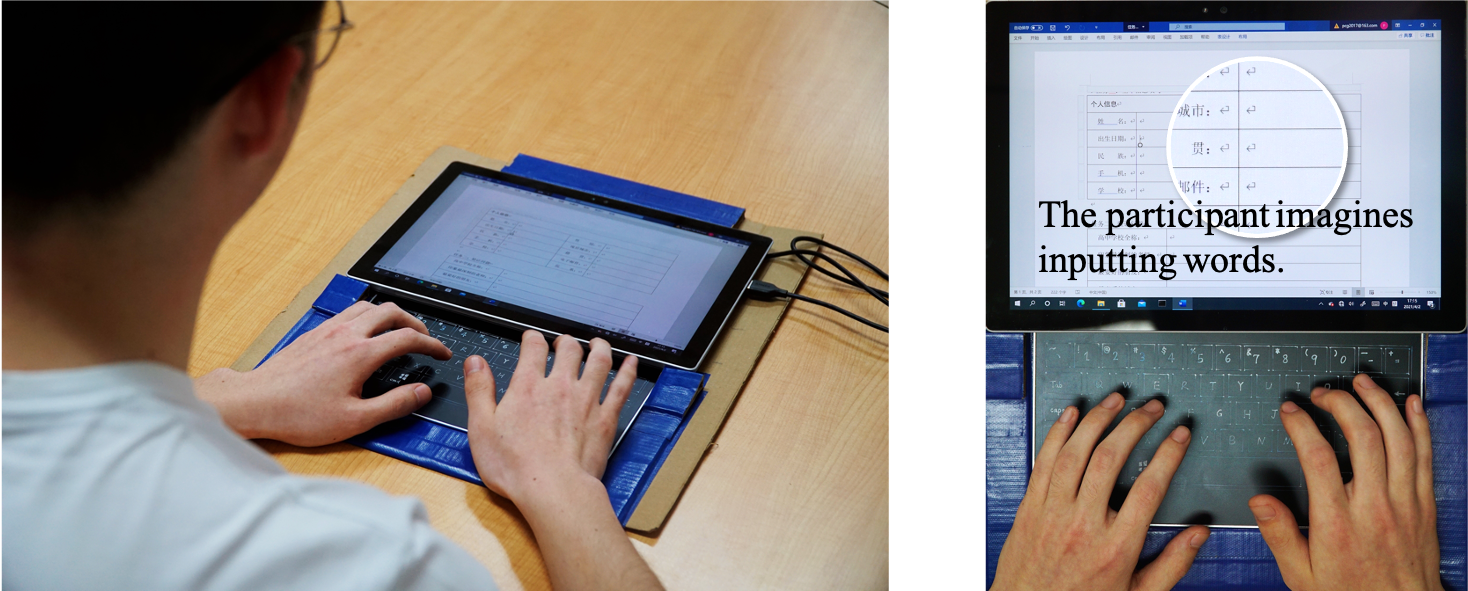
\includegraphics[width=0.9\linewidth]{figures/study1_illu.png}
	\centering
	\caption{The experimental setting of study one. We placed a tablet and a pressure-sensitive touchpad together as a substitute for the pressure-sensitive touchscreen. The keyboard had no feedback. The participant imagined inputting words.}
	\label{fig:study1_illu}
\end{figure}

The experiment included four text input tasks: (1) filling in personal information, (2) short questions, (3) open-book examination, and (4) picture writing. The tasks were in Chinese. We counterbalanced the order of tasks using a balanced latin square. We did not include transcription as a task as many other text entry studies do \cite{2003-Metrics, 2003-Phrase, 2017-Word}, because our pilot study showed that participants seldom rested their fingers on the touchpad in a transcription task, resulting in low efficiency of obtaining unintentional touches. The detail of tasks is as follows:

\begin{enumerate}
	\item{\textbf{Filling in personal information:} There was a table of ten blanks about personal information, such as name and gender. Figure \ref{fig:study1_task}(a) shows the examples in Chinese and the corresponding translation. This assignment represented those tasks that require frequent switching between text input and cursor control. To protect privacy, participants felt free to fill in fake information. However, participants should remember what they intended to input, which is crucial for the subsequent process of labeling data.}
	\item{\textbf{Short questions:} There was a table of ten short questions, such as "the favorite color" and "the best friend". Participants were allowed to fill in a fake answer.}
	\item{\textbf{Open-book examination:} The exam consisted of five hard questions, such as "what is the 50th element on the periodic table?". Participants could hardly know the answers, so they needed to search the Internet. This assignment represented the common task of browsing websites. Because the participants could not input words in the search engine, they said as they wrote, so the experimenter could replace them to input the words.}
	\item{\textbf{Picture writing:} As figure \ref{fig:study1_task}(b) shows, participants described the picture in five sentences. This assignment represented the tasks of writing articles. Participants said as they wrote, so the experimenter could replace them to input the words.}
\end{enumerate}

\begin{figure}[!tbh]
	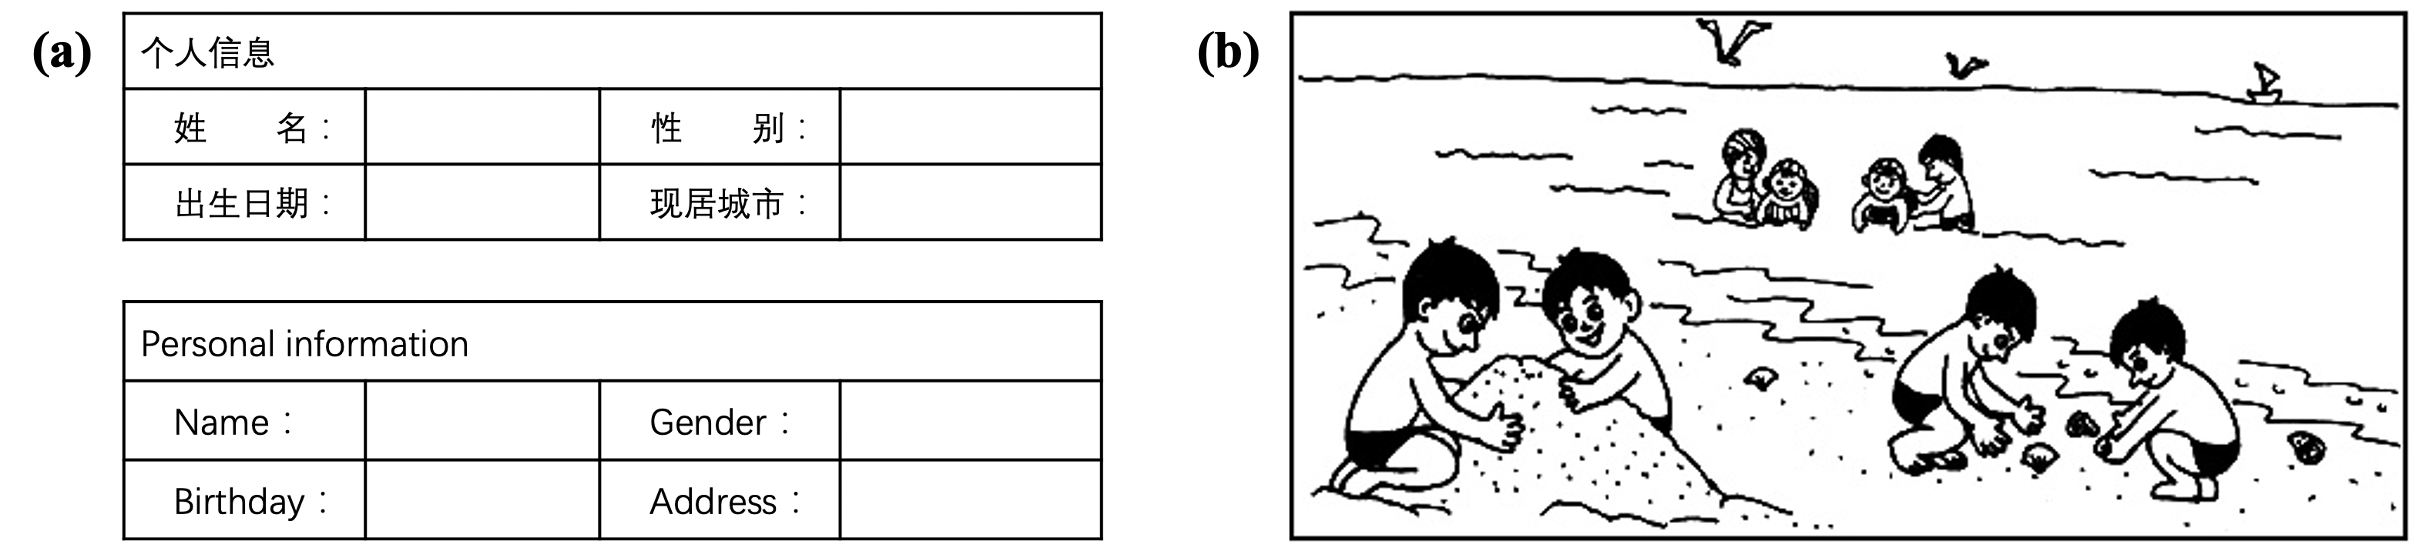
\includegraphics[width=0.9\linewidth]{figures/study1_task.png}
	\centering
	\caption{The illustration of experimental tasks. The left side shows the examples of task one (filling in personal information) in both Chinese and translation. The right side is the figure we used in task four (picture writing).}
	\label{fig:study1_task}
\end{figure}

Before the experiment, the participant had five minutes to get familiar with the experimental requirement. In the warm-up phase, participants typed on the touchpad freely. We reminded the participants of two points. First, the keyboard did not provide any feedback. Participants could not input words but imagined inputting words. As the Chinese text entry method involved word selection, participants assumed that the desired word is always the first in the candidate list. Second, users needed to imagine that the keyboard prevents unintentional touches and adjust their behavior according to this assumption. For example, they could rest their fingers on the keyboard while thinking.
%This is not mandatory. Participants could make choices as they wished.

%在实验开始前,用户有5分钟的时间自由地在本系统中熟悉实验的任务和要求,在热身的过程中,实验者让用户注意两点:第一,本实验的键盘不会提供任何反馈,用户不能键入字母,而是想象自己键入了字母。由于用户的母语是中文,在输入的过程中会涉及到选词,用户只需想象想要的单词总是在输入法候选词的第一位。第二,用户需要想象该键盘可以完美地防误触,并根据这一条件调整自己的输入行为,比如,在思考问题的时候可以将手指休息在键盘上。这种行为调整不是强制性的,用户可以根据自己的实际情况作出选择。

\begin{figure}[!tbh]
	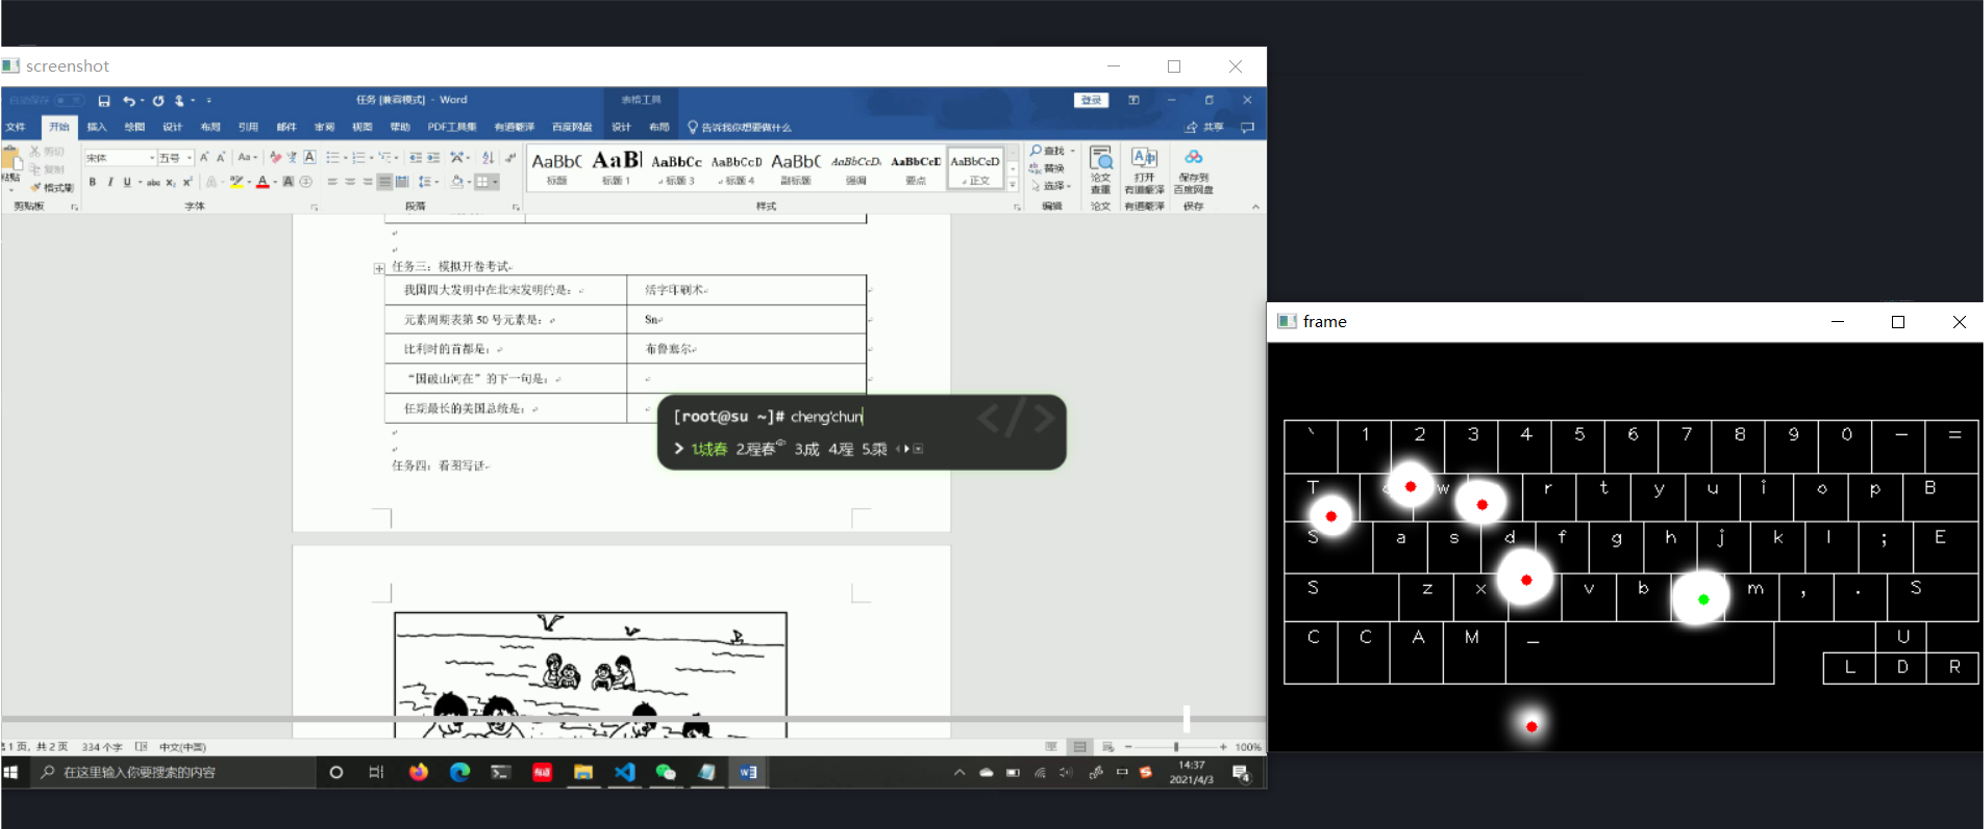
\includegraphics[width=1.0\linewidth]{figures/label_process.png}
	\centering
	\caption{The illustration of the label program.}
	\label{fig:label_process}
\end{figure}


After each task, the participant labeled the data through an interactive program as figure \ref{fig:label_process} shows. The program showed the touchpad capacitive images and the tablet screencast at the same time. There were red points on capacitive images that showed the touchpoints. Participants labeled the intended touches as green points. Participants were able to judge most touches because they could get context from the screencast. If participants were not sure, they labeled the touchpoints as blue points to remove the data. On average, participants spent five minutes finishing the text input tasks and spent 45 minutes labeling the data. Participants rested for five minutes between two tasks to avoid fatigue. The study lasted for 70 minutes.

\subsection{Apparatus}

As figure \ref{fig:study1_illu}(right) shows, we placed a Windows Surface tablet computer and a Sensel Morph pressure-sensitive touchpad \cite{Website-Morph} together as a substitute for the pressure-sensitive touchscreen. The Sensel Morph senses the position and the pressure level of touches. The Sensel Morph contains 185 x 105 sensor elements ("sensels") at a 1.25mm pitch. Each contact can sense approximately 30000 levels, ranging from 5g to 5kg. The maximal frequency of the Sensel Morph was 125Hz (8ms latency). We slowed the frequency down to 50Hz to fetch stable data. The Sensel Morph provides capacitive images and touchpoint information, including position, timestamp, touch area, pressure level, and shape. The device is so sensitive that almost every touch is recognized. Thus, in this paper, we identified unintentional touches among reported touchpoints while ignoring the Sensel Morph's missing touches.

The size of the sensing area on the Sensel Morph was 240 mm x 138 mm. We used highlighter pens to draw a Qwerty layout on the touchpad. The Sensel Morph width (240mm) was shorter than the keyboard on a 15 inches MacBook (270mm). We removed some keys that are less frequently used, such as square brackets and the semicolon, so that the Qwerty layout could be placed in the Sensel Morph, while each key's size remained the same as Macbook. Because the Qwerty layout is changeable in the software keyboard, we did not leverage the layout as prior knowledge to recognize unintentional touch. The tablet computer was Windows Surface Pro6, with i7 Intel Core Processor. The program ran on the tablet at 50 FPS.

\subsection{Result}

The dataset contains 12659 touches, excluding the ambiguous touches (0.18\%) in the labeling process. 67.5\% of the data were positive samples (intentional touches), while 32.5\% were negative samples (unintentional touches). Based on the data, we developed the TypeBoard in three steps, each contributing to solving one of the critical problems as follows:

\begin{enumerate}
	\item{\textbf{Model V1):} \emph{data processing.} There were some mislabeled data points because some participants misunderstood the concept of unintentional touches. We developed a naive Support Vector Machine (SVM) model to identify unintentional touch. If there was a vast difference between the predicting results and the labels, we asked the participants to relabel the suspicious data points through e-mails.}
	\item{\textbf{Model V2):} \emph{filtering multiple fingers resting.} Observation suggested that multiple fingers resting was the most frequent unintentional touch, where users rested more than two fingers on the screen. We added targeted criteria into the SVM model to filter out multiple fingers resting.}
	\item{\textbf{Model V3):} \emph{understanding the user behavior.} We analyzed the fail cases of Model \textbf{V2} to understand those user behaviors that challenged the algorithm, based on which we further improved the SVM model.}
\end{enumerate}

\begin{table}[!tbh]
	\caption{The features we fed into the SVM model and the accuracy among model versions. For the features except "the relationship to recent/nearby touches", we extracted the temporal features over frames, including maximum, minimum, mean, skewness, and kurtosis.}
	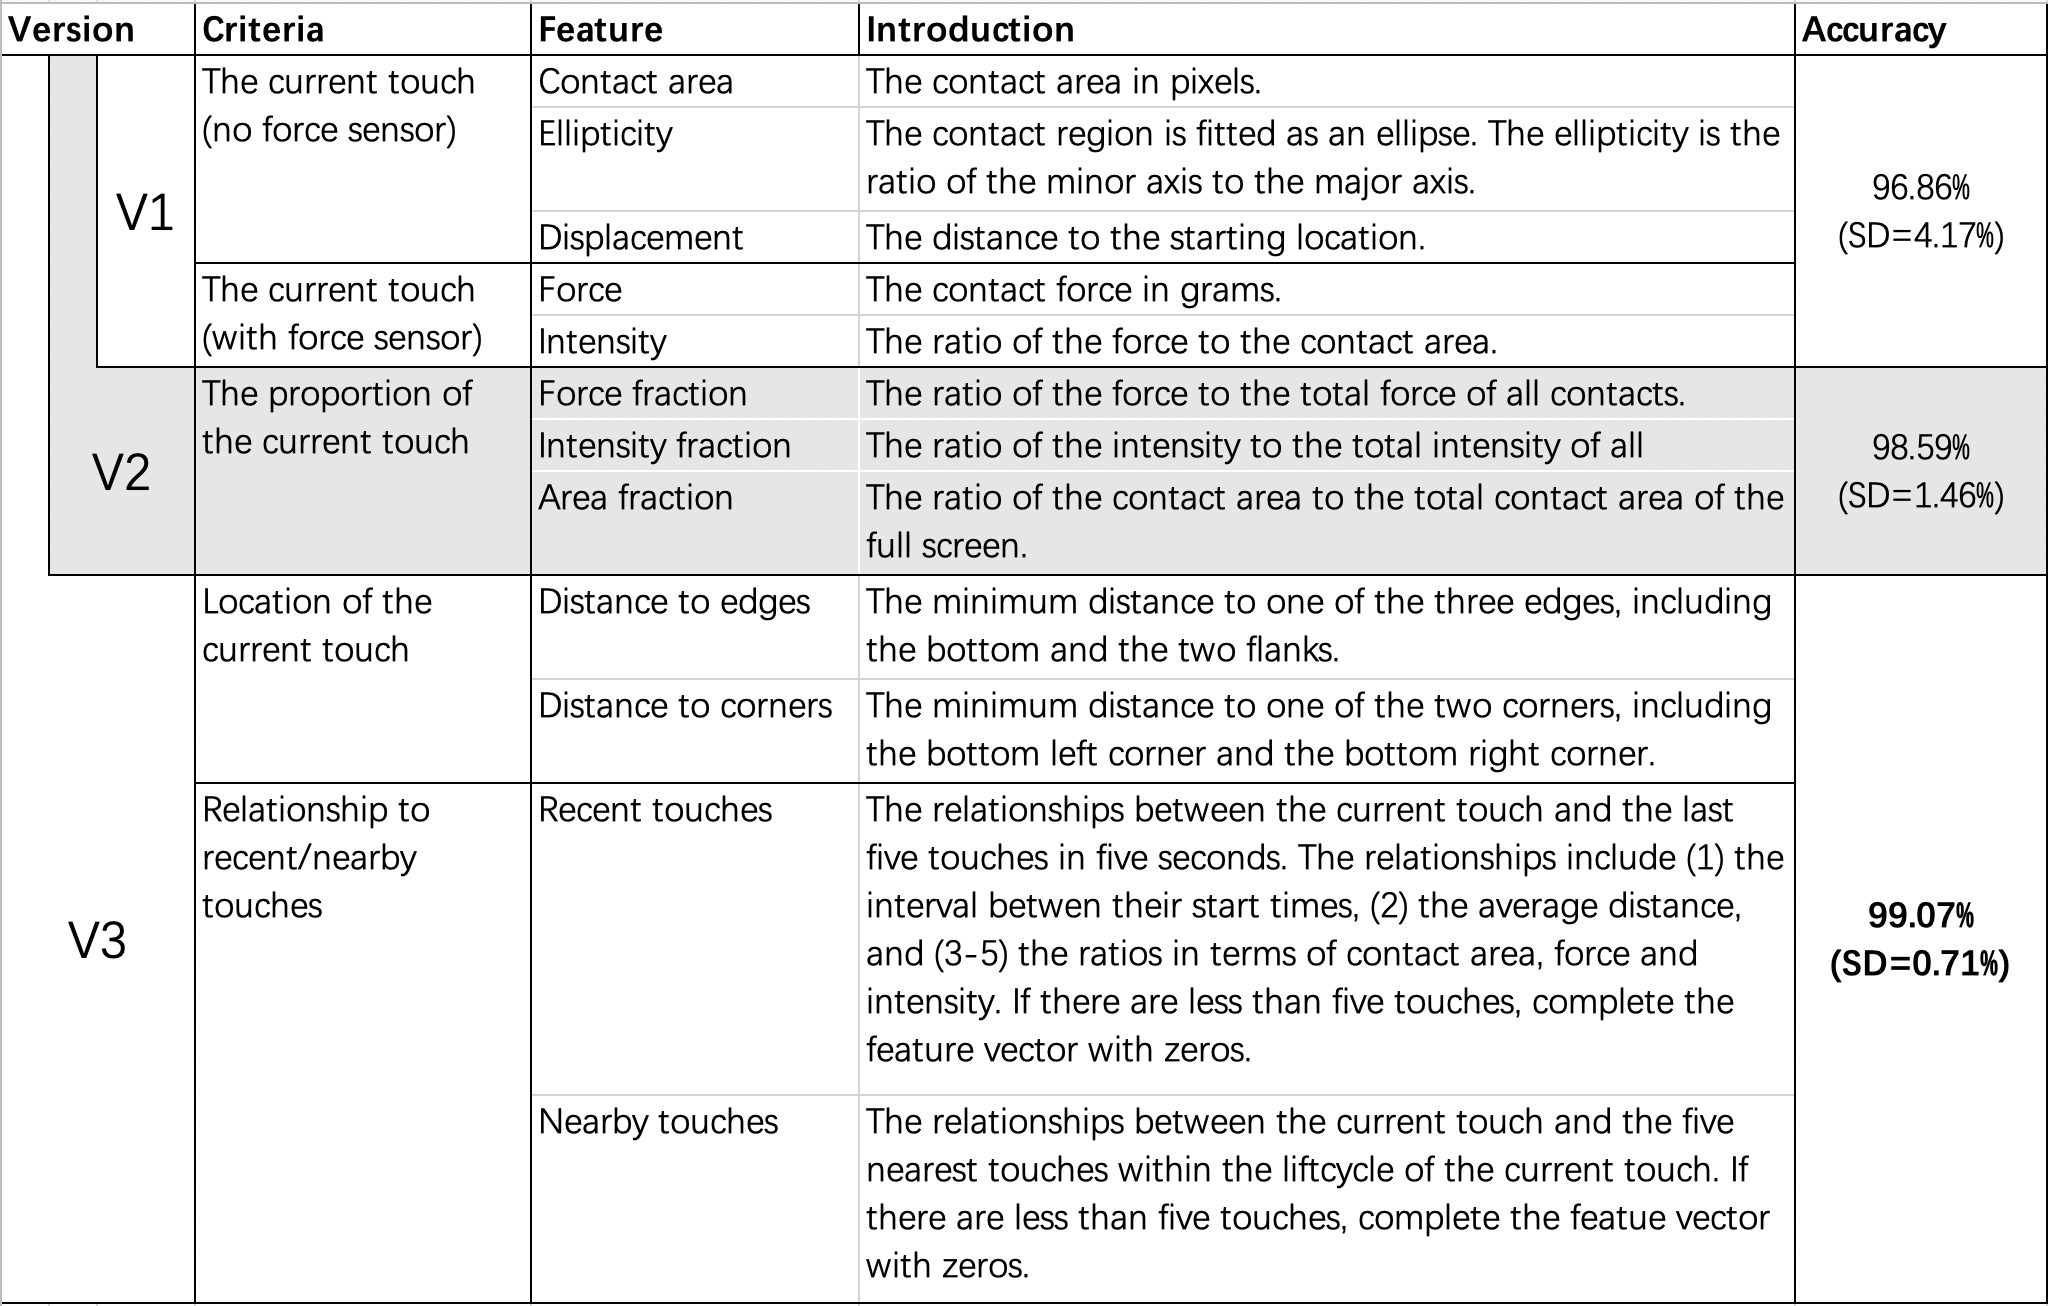
\includegraphics[width=1.0\linewidth]{figures/features.png}
	\centering
	\label{tab:study_features}
\end{table}

Table \ref{tab:study_features} shows the feature vector we used to train the SVM model in each step and the recognition results. In the remainder of this subsection, we introduced the unintentional touch identification model in detail.

%Because some participants misunderstood the concept of unintentional touches when labeling, there were some mislabeled data points. We trained a simple machine learning model (version 1) to process the data. If there were too many differences between the labels and the predicting results, we asked the participants to relabel the suspicious data points.

\subsubsection{Model  V1: naive model for data processing}

In the first step, we trained a naive SVM model to identify unintentional touch using straightforward features. We sampled the first five frames (100 ms) of each touch. If the touch duration is shorter than five frames, we sampled the whole touch. As table  \ref{tab:study_features} (\textbf{V1}) shows, we extracted features from the samples as follows: for the contact area, ellipticity, displacement, force, and intensity over frames, we calculated the temporal features, including maximum, minimum, mean, skewness, and kurtosis. Then, we concatenated these values to obtain a feature of 25 dimensions and trained an SVM binary classifier, namely Model \textbf{V1}. We balanced positive and negative samples in weight.

We used the model to simulate the dataset. We found that some participants misunderstood the concept of unintentional touches, for example, regarding incorrect character inputs as unintentional touches. We asked the participants to relabel the suspicious data points through e-mail. After the label correction, we had 12624 data points, including 68.38\% positive samples and 31.62\% negative samples. Leave one out cross-validation shows that the accuracy of Model \textbf{V1} was 96.86\% (SD=4.17\%). 

%For comparison, if we did not have the force signal (i.e., the regular touchscreen devices), the accuracy would reduce to 92.30\% (SD=4.88\%). The result shows that the force signal is important for unintentional touch rejection (F,p).

\subsubsection{Model V2: filtering multiple fingers resting}

Observation showed that most unintentional touches (72.66\%) were caused by multiple fingers resting, where users rested no less than three fingers on the screen simultaneously. The resting fingers contact the screen one after another. After the first touch, the following touches come within 100 ms in most instances. In 86.05\% cases, the second finger touches within 100 ms, while in 76.30\% cases, the third finger also touches within 100 ms. Because our model has a latency of 100 ms, the model has a big chance to realize that multiple fingers are resting. Thus, we could design targeted features to filter out the unintentional touches caused by multiple fingers resting.
We added a series of features in Model \textbf{V2} to deal with this problem. The criterion was the proportion of the touch's pressure, intensity, and contact area among all touches. Table \ref{tab:study_features} (\textbf{V2}) shows the details. Leave one out cross-validation shows that Model \textbf{V2} increased the recognition accuracy to 98.59\%.

\subsubsection{Model V3: understanding the user behavior to  improve the model}

We analyzed the fail cases of Model \textbf{V2} to understand those user behaviors that challenged the model. The error rate of Model \textbf{V2} was 1.41\%, including 1.00\% false positives and 0.41\% false negatives. The false positives referred to the misrecognized unintentional touches, while the false negatives were the missing intentional touches. As table \ref{tab:fail_cases} shows, we classified the fail cases into 16 categories. We counted each kind of fail case, discussed the reasons, and gave possible solutions. For the fail cases with a white background in the table, humans (the researchers) could judge their intentions without extracting contextual information from the experiment screencast. That is, the machine should have correctly predicted if it is as smart as a human. For these cases, we proposed features to improve the model. Here are some examples.

\begin{enumerate}
	\item{\textbf{EG1):} \emph{Hypothenar eminence.} As figure \ref{fig:fail_case_examples}(a) shows, the hypothenar eminence refers to a group of muscles of the palm that control the motion of the little finger, while the thenar eminence is the group of muscles on the palm at the base of the thumb. Both the two eminences may contact the touchscreen when a user is typing. In particular, the touches caused by the hypothenar eminence are usually heavy and intensive, which is easy to confuse with intentional touches. Fortunately, these touches are in the bottom left and the bottom right corners. Thus, the distance to the closest corner could be a powerful feature to reject these unintentional touches.}
	\item{\textbf{EG2):} \emph{Continuous touches.} When a user continuously typed on the same key (e.g., the backspace), the following touches were lighter than the first touch (p < 0.005). Among the continuous touches, the average pressure of the first touch was 167.01 g (SD = 106.76), while the average pressure of the following touches was 150.42 g (SD = 112.70). Because the following touches are light, they are likely to be recognized as unintentional touches. Information of recent touches help to correct this fail case.}
	\item{\textbf{EG3):} \emph{One-hand typing.} As figure \ref{fig:fail_case_examples}(b) shows, sometimes the participant typed with one hand while resting the other hand on the touchscreen. In this situation, the Model \textbf{V2} mistakenly believed that all the touches were unintentional touches caused by the multiple fingers resting behavior. We added information of nearby touches to correct this fail case because the typing finger is usually far away from the resting fingers.}
\end{enumerate}

\begin{figure}[!tbh]
	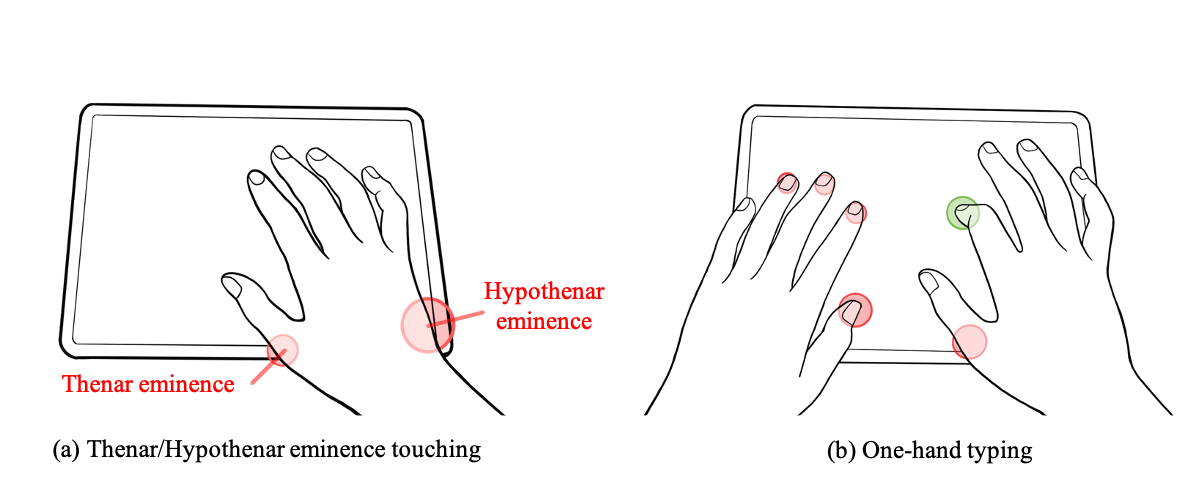
\includegraphics[width=1.0\linewidth]{figures/fail_case_examples.png}
	\centering
	\caption{The examples of fail cases. The fail cases reveal those user behaviors that challenged the algorithm.}
	\label{fig:fail_case_examples}
\end{figure}

% Table generated by Excel2LaTeX from sheet '写在论文中的中等粒度分类'
\begin{table}[htbp]
  \centering
  \caption{The fail cases of Model \textbf{V2}. The "N" column refers to the counting of each case.}
    \begin{tabular}{|p{8.5em}|p{21em}|r|p{10.5em}|}
    \toprule
    \textbf{Cases} & \textbf{Introduction} & {\textbf{N}} & \textbf{Helpful features?} \\
    \midrule
    \rowcolor[rgb]{ 1,  .902,  .6} \multicolumn{4}{|l|}{\textbf{False Positives}} \\
    \midrule
    Hypothenar eminence (figure \ref{fig:fail_case_examples}a) & The hypothenar eminence usually contacts the screen while typing. & 23    & Touchpoint location, e.g., nearing the corners? \\
    \midrule
    Thenar eminence (figure \ref{fig:fail_case_examples}a) & The thenar eminence usually contacts the screen while typing. & 2     & Touchpoint location, e.g., nearing the bottom edge? \\
    \midrule
    Repeated reporting (spatial) & A touch is misrecognized as two touches when the contact area is large. & 12    & Info. of nearby touchpoints. \\
    \midrule
    Repeated reporing (temporal) & A touch is misrecognized as two touches if the touch is nearly released midway. & 3     & Info. of recent touchpoints. \\
    \midrule
    Edge touch & Users trigger unintentional edge touch when adjusting the placement of devices. & 7     & Touchpoint location, e.g., nearing the flanks? \\
    \midrule
    Two fingers resting & The user rests two fingers on the screen. & 3     & Info. of nearby touchpoints. \\
    \midrule
    Extra touchpoint (light) & When inputting, users trigger extra touchpoints, which are lighter than the recent intentional touches. & 9     & Is this touch lighter than the recent touches? \\
    \midrule
    Slide & A slide is less likely to be an intentional keystroke. & 7     & Touchpoint displacement. \\
    \midrule
    \rowcolor[rgb]{ .949,  .949,  .949} One finger resting & Users rest one finger on the touchsreen, which is indistinguishable from an intentional touch. & 9     & No solution. \\
    \midrule
    \rowcolor[rgb]{ .949,  .949,  .949} Extra touchpoint (heavy) & When inputting, users trigger extra touches heavily, which seems like an intentional touch. & 15    & No solution. \\
    \midrule
    \rowcolor[rgb]{ 1,  .902,  .6} \multicolumn{4}{|l|}{\textbf{False Negatives}} \\
    \midrule
    Continuous touches & When a user continuously type on the same key (e.g., the delete key), the following touches will be lighter. & 13    & Info. of recent touchpoints. \\
    \midrule
    Rollover-typing & The next key is pressed before the previous is released \cite{2018-Observations}. & 12    & info. of recent touchpoints. \\
    \midrule
    One-hand typing & The user types with one hand, while the other hand is resting on the screen. This case is similar to multiple fingers resting. & 6     & info. of nearby touchpoints. \\
    \midrule
    Palm touch & The use types a key when the palm is resting on the screen. If the palm touch is detected as multiple fingers, this case is similar to multiple fingers resting. & 5     & info. of nearby touchpoins, e.g., is this touch near other touches? \\
    \midrule
    \rowcolor[rgb]{ .949,  .949,  .949} Light touch & The very light but intended touch, which is indistinguishable from an unintentional touch. & 46    & No solution. \\
    \midrule
    \rowcolor[rgb]{ .949,  .949,  .949} Small contact area & The intended touch with a very small contact area. This seems like an unintentional touch. & 6     & No solution. \\
    \bottomrule
    \end{tabular}%
  \label{tab:fail_cases}%
\end{table}%

However, for the fail cases with gray background in table \ref{tab:fail_cases}, humans (the researchers) could judge their intentions without watching the experiment screencast. We deemed that these fail cases are inevitable because the machine can not know what the user will input in advance. Here are some examples. First, sometimes the participant rested one finger on the touchscreen heavily, indistinguishable from an intentional touch. Second, the participant performed a very light touch during inputting a word, which is indistinguishable from an unintentional touch. Thus, the model's accuracy has a certain upper limit (roughly 99.40\% in this dataset), while our goal is to approach it.

According to the user behaviors summarized in table \ref{tab:fail_cases}, we added two criteria in the model training. The first one is the location of the touch, including the minimum distances to the edges and the corners. We did not leverage the prior knowledge of the keyboard layout because the software keyboard layout is changeable, while we wanted a universal model. The second criterion is the relationships between the current touch and the recent/nearby touches. The features in detail are in table \ref{tab:study_features} (\textbf{V3}). The Model \textbf{V3} used all the features in the table. We concentrated these features to form a vector of 100 dimensions and trained an SVM binary classifier. Leave one out cross-validation showed that the accuracy was 99.07\%. The error rate was 0.93\%, including 0.56\% false positives and 0.37\% false negatives. So far, we have obtained a model with high recognition accuracy. However, as we said in the introduction, the data collected in study one did not represent the user behavior on the software keyboard with unintentional touch prevention, so we named Model \textbf{V3} as semi-finished TypeBoard. In study two, we collected the user behavior on the semi-finished TypeBoard and then used the new data to improve the model.

% We used previous work as baseline \cite{2013-TapBoard}, where every touches that last for more than 450 ms or move father than 15 mm are identified as unintentional touches. We adjusted the thresholds to yy ms and yy mm so that the baseline performed the best on our dataset. Our result (99.07\%) surpassed the baseline (yy\%). In real use, our system calls the classifier once a touch has lasted for five frames or is released in advanced. The system reports the touchpoint if the prediction result is positive. The delay of our method is 100 ms. For comparison, the baseline can only judge a touch when it is released.

%We have three conclusions in this experiments. First, participants were willing to rest their fingers on the touchscreen that can reject unintentional touches in imaginary. Hereby, we proposed a hypothesis to be verified, where users are willing to rest their fingers on a real TypeBoard. Second, the force signal is important for rejecting unintentional touches in the text entry task. Third, most unintentional touches (>99\%) can be identified by spatial-temporal features of the signals on a force-sensitive touchsreen keyboard.



\section{Study 2: User Behavior on the TypeBoard}

In this study, we obtained users' typing data on the TypeBoard, which is a touchscreen keyboard with unintentional touch rejection. The motivation was to investigate users' typing behavior, based on which we can improve the identification of unintentional touch. We have implemented a TypeBoard in the last study. In this study, we recruited 16 participants and divided them into four groups equally. The first group of participants typed on the existing TypeBoard. After each group finished the experiment, we used the data to improve the TypeBoard. The following participants typed on the improved TypeBoard. That is, we explored the user behavior and improve the method through an iterative process.

%在本实验中,我们迭代地采集了用户在防误触触屏键盘上的打字数据。动机是调研用户在防误触触屏键盘上的打字行为,基于此我们可以优化防触屏键盘上的防误触算法。在实验一中,我们已经得到了一个naive版本的TypeBoard(防误触键盘)。在本实验中,我们邀请5组*4人=20人在TypeBoard上打字,在每采集完4名被试的数据之后,我们都会利用新的数据去优化TypeBoard,并让后续的用户在优化后的TypeBoard上进行实验。这样做的目的是通过迭代的方法来逼近鲁棒的防误触算法,和探索其上的用户行为。

\subsection{Participants}

We recruited 20 participants from the local campus (aged from xx to xx, M = xx.xx, SD = xx.xx, xx femakes). All the participants were righted handed and did not took part in the first study. They have used software keyboards on smartphones for not less than xx years. xx of the 20 participants were familiar with software keyboards on tablets.

We divide the participants into five groups. Each group had four people. The five groups were well-matched in age. As a previous work did \cite{2020-QwertyRing},  we ran a program to divide the participants randomly for 1000 times and picked the five groups of which the average ages were the closest (M = xx.x, xx.x, xx.x, xx.x, xx.x, SD = xx.x, xx.x, xx.x, xx.x, xx.x). The first group of participants typed on the naive TypeBoard, while the following groups used continually improved keyboards.

%我们从本地的校园中邀请了20名用户参与实验,他们的年龄从xx岁到xx岁不等,平均数是xx,标准差是xx,其中有xx名女性。所有的用户都是右撇子,所有用户有超过xx年的手机文本输入经历,xx名用户常用平板电脑进行文本输入。这些用户没有参与过实验一。如上面所说,我们将用户分成了五组,为了保证五组用户的平衡性,我们通过程序随机模拟了10000次分组,最终确定了平均年龄最相近的分组方式,这五组的年龄平均数分别为xx,xx,xx,xx,xx,每组分别有xx,xx,xx,xx,xx名女性。

\subsection{Design and Procedure}

As figure xx shows, the experimental devices were the same as those in study one, including a Windows surface tablet and a Morph Sensel force-sensitive touchpad. The working frequency was 50 FPS. There were four sessions of text entry tasks, which also reminded the same as study one. The differences in study two are as follows. First, participants could actually enter words by typing on the touchpad. Second, the system supported unintentional touch rejection. Intentional touches would trigger keystrokes and audio feedback, while unintentional touches were ignored.
%正式实验分为四个session,分别收集了用户在填写个人信息、描述个人爱好、模拟开卷考试和看图写话这四个任务下的打字数据,我们通过拉丁方来平衡每个用户做这四个任务的顺序。如图xx所示展示了实验二的实验设置,桌面上的实验设备包含morph-sensel压力触摸板、鼠标、显示器和耳机。在本实验中,用户同样通过填写word文档的方法来完成四个文本输入任务(图xx)。和实验一不一样的是,用户在本实验中真的能够通过TypeBoard来键入字母,且打字的过程中能够听到“啪啪”的声音反馈。

Before the experiment, participants warmed up by a ten-minute daily writing. Because no participant had experience with typing on a keyboard with unintentional touch rejection, we reminded the participants that they could rest their fingers on the keyboard while thinking. The resting behavior was not mandatory. Participants could decide to rest or not according to the task and their preference.

%在实验之前有一个训练阶段,用户有五分钟时间通过誊写例句熟悉该键盘,例句随机选自xx例句库[xx]。由于所有用户都没有过使用防误触触屏键盘的体验,在用户的试用过程中,实验者提醒用户该键盘有防误触的功能,平时可以把手休息在触屏上。这不是强制的要求,具体行为由用户根据具体的任务和自己的喜好决定。

In rare cases, the system repeatedly ignored participants' intentional touches. For example, a participant (px) usually typed with one hand while the other hand rested on the touchsreen. This behavior was not observed in study one, so the system could not identify it correctly. Considering that these fail cases were useful to improve the unintentional rejection algorithm, we encouraged the participant to keep their behaviors when the system gave an incorrect response. In this situation, participants needed to imagine that the desired words were corrected entered.

%在极少数情况下,用户会发现一类机器学习总是错判的情况,字母不能正常上屏。举例来说,第x名用户经常在单手五指都休息的情况下,另一只手打字,系统总是漏报。在这种情况下我们鼓励用户维持这种系统会误判的用户行为,并像实验一中一样想象字母已经正确上屏,然后在标注的时候标注出这些错误。

After finishing each session, participants labeled the data through an interactive program, which was introduced in study one. During the labeling phrase, we compared participants' labels with the results predicted by the algorithm. When the two results were different, we immediately recorded and analyzed the data point. If the experimenter could not figure out why the results were different, he would discuss with the participant.
In average, participants spent 10 minutes to finish the text entry tasks and spent one hour to label the data. The completion time was longer than that in study one, because participants needed more time to enter and correct words in study two. Participants rested for five minute between two sessions to avoid fatigue. The study was generally completed within 90 minutes.

%在每个session结束后,用户通过交互式程序标注刚刚完成的session的报点。和实验一的标注过程相同,所有的报点一开始都被标为红色(误触),用户需要将每一个有意的点击标注成绿色(正例)。实验者在一旁观察标注的过程,并通过另一台电脑事先得知机器学习的结果,当发现机器学习结果和用户人工标注不符的情况时,实验者会人工分析其中的原因,如果实验者不能通过独立思考弄明白其中的原因,或者他认为被试标注出错时,他会立即和被试进行讨论。

%在本实验中,用户完成输入任务的总时间大约为30分钟,比实验一稍长,这是因为实验二的输入过程涉及键入字母和删改操作;用户完成标注的时间大约为45分钟;每两个session之间用户休息5分钟时间以避免疲劳,实验总时长为90分钟。

Because the ability of unintentional touch rejection will affect the user behavior, we used an iterative process to improve TypeBoard, and ensured that the participants were typing on the latest version of TypeBoard. We divide the 16 participant into four groups. The first group of participants complete the experiment on the naive TypeBoard introduced in study one. After each group of participants finish their experiment, we improved the algorithm by updating training data and adding features in model. We expected that the TypeBoard algorithm was getting stronger, while the data we collected was getting closer to the natural behaviors of typing on a perfect keyboard.

%由于用户的打字行为和触屏防误触能力会互相影响,我们将20名被试平均分为五组,在每组被试完成实验后,我们都会更新数据集和添加必要的特征向量,以训练新的防误触算法,迭代地增强触屏键盘的防误触能力。这就是说,我们期望每组用户所用到的TypeBoard键盘的防误触能力都会更强,也期望每组用户的打字行为更接近防误触键盘上的自然输入行为。

\subsection{Result: Recognition}

在实验的过程中,每四个用户的实验结束之后,我们都会采用新的数据来优化防误触算法,如图xx所示是防误触算法随着完成实验人数的增加的变化,其中每个测试点的数据集包含实验二过程中已经收集到的数据加上实验一的所有数据,评测方法是leave-one-out检测。结果表明,随着实验人数的增加,迭代更新TypeBoard和初版TypeBoard的差距在显著拉大。这说明TypeBoard的防误触能力在增强,我们采集到的数据也越来越接近用户在一个完美防误触键盘上的打字行为。

【图:baseline、初版TypeBoard、迭代更新TypeBoard随着实验人数增加,准确率的变化】

在16名用户的实验都完成了之后,抛去用户无法区分的xx个数据点,我们共收集了xx个有效的数据点。在经过了和实验一相同的label结果确认之后,数据集中正例(打字)的比例是xx.x\%,负例(误触)的比例是xx.x\%。如表格xx所示,我们总结了一些初版模型fail cases,我们针对这些情况专门设计了额外的特征组。至此,我们完成了TypeBoard的最终设计,特征向量是xx维,我们的算法在实验二的数据集上达到了xx.x\%的准确率。

【表:实验二新总结出来的fail-cases和应对方案】

上述是在高精度的force-sensitive touchscreen keyboard上的识别结果,其准确率较高。然而,现实中大多数触摸屏设备还没有压力传感器,有的设备(如MacBook的force touch trackpad)则在四个角上有压力传感器。为了给防误触触屏提供硬件设计指导,我们对比了我们的算法在三种情况下识别准确率,三种情况分别是:(1)capactive-only:只有电容信号;我们将算法中涉及到压力信号的特征维度都阉割掉来训练机器学习模型。(2)four-force-sensor:四个角上有压力传感器,根据实验采集到的高精度压力信号,我们可以根据基础的物理知识模拟四角压力传感器的数据。我们在情况1的基础上,直接加上四个角压力信号的时域特征。(3)force-enabled:既有电容信号,又有压力信号,这也就是我们论文中所述的配置。

【图:三种硬件设置下算法的识别准确率】

如上图所示是这三种情况下算法的识别准确率。值得注意的是,四个角上有传感器的识别准确率为xx.xx\%,这说明,四个角上安装传感器是一个准确率不错、且目前为止容易实现、成本较低的实现方法。

\subsection{Result: User Behavior}

在本实验的结果中,我们更多地关注在用户的行为上。

(1)误触点的构成:休息、手掌误触、输入时误触的比例。

(2)实验任务显著影响了用户行为。这说明了考虑不同实验任务的必要性。

(3)技术实现和用户行为之间的互相影响,及应对方案。可以列举很多相关工作进行讨论,比如其它防误触算法、文本输入相关算法。


\section{Study 3: Evaluation on TypeBoard}

实验三的目的有两点:第一,评测TypeBoard的性能,包括在不同的文本输入任务下的输入效率和主观用户体验,baseline是没有防误触算法的触屏键盘。第二,相关工作中我们提到,在防误触触屏键盘上,有望通过加上纹理反馈帮助用户盲打,提高输入效率,本实验探索了这一假设是否成立。

\subsection{Design and Procedure}

我们从本地的校园中邀请了15名用户参与实验,他们的年龄从xx岁到xx岁不等,平均数是xx,标准差是xx,其中有xx名女性。所有的用户都是右撇子,所有用户有超过xx年的手机文本输入经历,xx名用户常用平板电脑进行文本输入。这些用户没有参与过前两个实验。

我们采取了within-subject的实验方法,对比了三种不同的实验设置(如图xx所示):第一种设置,普通的触摸屏键盘;第二种设置,TypeBoard算法+整张的Qwerty布局贴纸,这也是实验二的设置;第三种设置,TypeBoard算法+沿着每个按键模切的Qwerty布局贴纸,其中F键和J键上和物理键盘上一样有额外的触觉反馈。贴纸的厚度是xx毫米,用户可以摸到每个键的边缘。每名用户依次使用这三种实验设置来完成前两个实验中提到的五种文本输入任务。为了平衡学习效应,我们采用拉丁方来规定用户使用这三种实验设置的顺序。

【图:实验三要对比的三种实验设置】

用户使用每一种实验设置之前,都用5分钟的热身时间,通过输入例句来热身。用户在切换实验设置的时候休息5分钟时间,以避免疲劳。用户在每个实验设置下需要完成与实验二相同的五个文本输入任务,每种实验设置下的实验时长大约为xx分钟。实验的总耗时为xx分钟。

\subsection{Appartus}

除了触摸屏存在三种不同的设置以外,其余设备与实验二完全一样。桌面上只有触摸板和显示器这两种设备,用户通过耳机来获取打字瞬间的声音反馈。

\subsection{Result}

要注意的点:
1. 有无landmarks两种情况下,用户盲打的时间对比;每个按键点云标准差的对比;误触数量的对比;错误率。

我们采用了什么样的统计分析方法,对于xx等违反正态分布的量,我们通过xx方法来进行校正。如果一个独立变量对结果有显著性影响,我们采用xx方法来检验变量两两之间的显著性。

\subsubsection{Completion Time}

English.

在誊写任务下可以对比打字速度。

\subsubsection{Error Rate (Text Entry)}

CER

UER

\subsubsection{Detected Unintentional Touches Percentage}

\subsubsection{Time Components}

\subsubsection{Subjective Rating and Feedback}

\subsubsection{Percentage of EyeFree time}

\subsection{Discussion}

\subsubsection{TypeBoard vs. Regular Board}

English.

对用户行为、用户体验、输入效率的影响。

\subsubsection{TypeBoard with/without tactile feedback}

English.

对用户行为、用户体验、输入效率的影响。


\section{Discussion}


\section{Limitation and Future Work}

\subsection{Limitation}

\subsection{Future Work}

有可能的follow up works:

键盘、触摸板一体for个人笔记本电脑?

触屏+纹理=触屏盲打?

利用手掌位置来处理触屏输入法中的漂移问题。


\section{Conclusion}

一些结论。

\bibliographystyle{ACM-Reference-Format}
\bibliography{acmart}

\end{CJK*}
\end{document}
\endinput
%%
%% End of file `sample-acmlarge.tex'.
